\documentclass[dvipdfmx]{jsarticle}
\usepackage{amsmath,amsfonts}
\usepackage{titlesec}
\usepackage{graphicx}
\usepackage{float}
\usepackage{comment}
\usepackage{fancyhdr}
\usepackage{url}

\lhead{}%ヘッダ左上を空白化
\graphicspath{{../fig/}}%\includegraphicsのファイル名省略用
%高さの設定
\setlength{\textheight}{\paperheight}%ひとまず紙面を本文領域に
\setlength{\topmargin}{-5.4truemm}%上の余白を20mm(=1inch-5.4mm)に
\addtolength{\topmargin}{-\headheight}%
\addtolength{\topmargin}{-\headsep}%ヘッダの分だけ本文領域を移動させる
\addtolength{\textheight}{-40truemm}%下の余白も20mmに
%%幅の設定
\setlength{\textwidth}{\paperwidth}%ひとまず紙面を本文領域に
\setlength{\oddsidemargin}{-0.4truemm}%左の余白を20mm(=1inch-5.4mm)に
\setlength{\evensidemargin}{-0.4truemm}%
\addtolength{\textwidth}{-50truemm}%右の余白も20mmに

%図,表の表示名
\renewcommand{\figurename}{Fig. }
\renewcommand{\tablename}{Table }

%図,表,式などの間隔
\setlength{\abovecaptionskip}{1mm}	%図・表とキャプションの間隔の変更
\setlength{\belowcaptionskip}{1mm}
\setlength{\abovedisplayskip}{3pt}%式の上部のマージン
\setlength{\belowdisplayskip}{3pt}%式の下部のマージン

%図番号を(subsection).(図番号)に変更
\makeatletter
\renewcommand{\thefigure}{\thesection.\arabic{figure}}
\@addtoreset{figure}{section}

%表番号を(subsection).(表番号)に変更
\renewcommand{\thetable}{\thesection.\arabic{table}}
\@addtoreset{table}{section}

%式番号を(subsection).(式番号)に変更
\renewcommand{\theequation}{\thesection.\arabic{equation}}
\@addtoreset{equation}{section}
\makeatother

%注釈
\renewcommand\thefootnote{*\arabic{footnote}}

%目次の表示レベル設定
\setcounter{tocdepth}{3}


\renewcommand{\postpartname}{章} %部を章に変更
%\renewcommand{\thepart}{\Roman{part}}  

\begin{document}

\twocolumn[
  \begin{center}
    \vspace{20mm}
    {\huge 研究計画書}\\
    \vspace{5mm}  
    {\Large 車輪に依存しない段差踏破ロボットの開発}\\
    \vspace{5mm}
    {\Large 千葉工業大学 先進工学部 未来ロボティクス学科 米田研究室}\\
    {\Large 学生番号 21C1016 稲葉健}\\
    \vspace{5mm}
    {\Large \today}\\
  \end{center}
]

\section{研究背景}
近年普及の進む掃除ロボットを始めとする室内移動系のロボットは、車輪径・車高を大きくすることが難しいケースも少なくない。
しかし、一般的な車輪ロボットでは、車輪半径の半分以上、車高以上の段差を登攀することは困難である。
そのため、現行の室内移動ロボットの運用は、大きな段差のないフロアを移動することが主である。

% 画像
\begin{figure}[htbp]
  \centering
  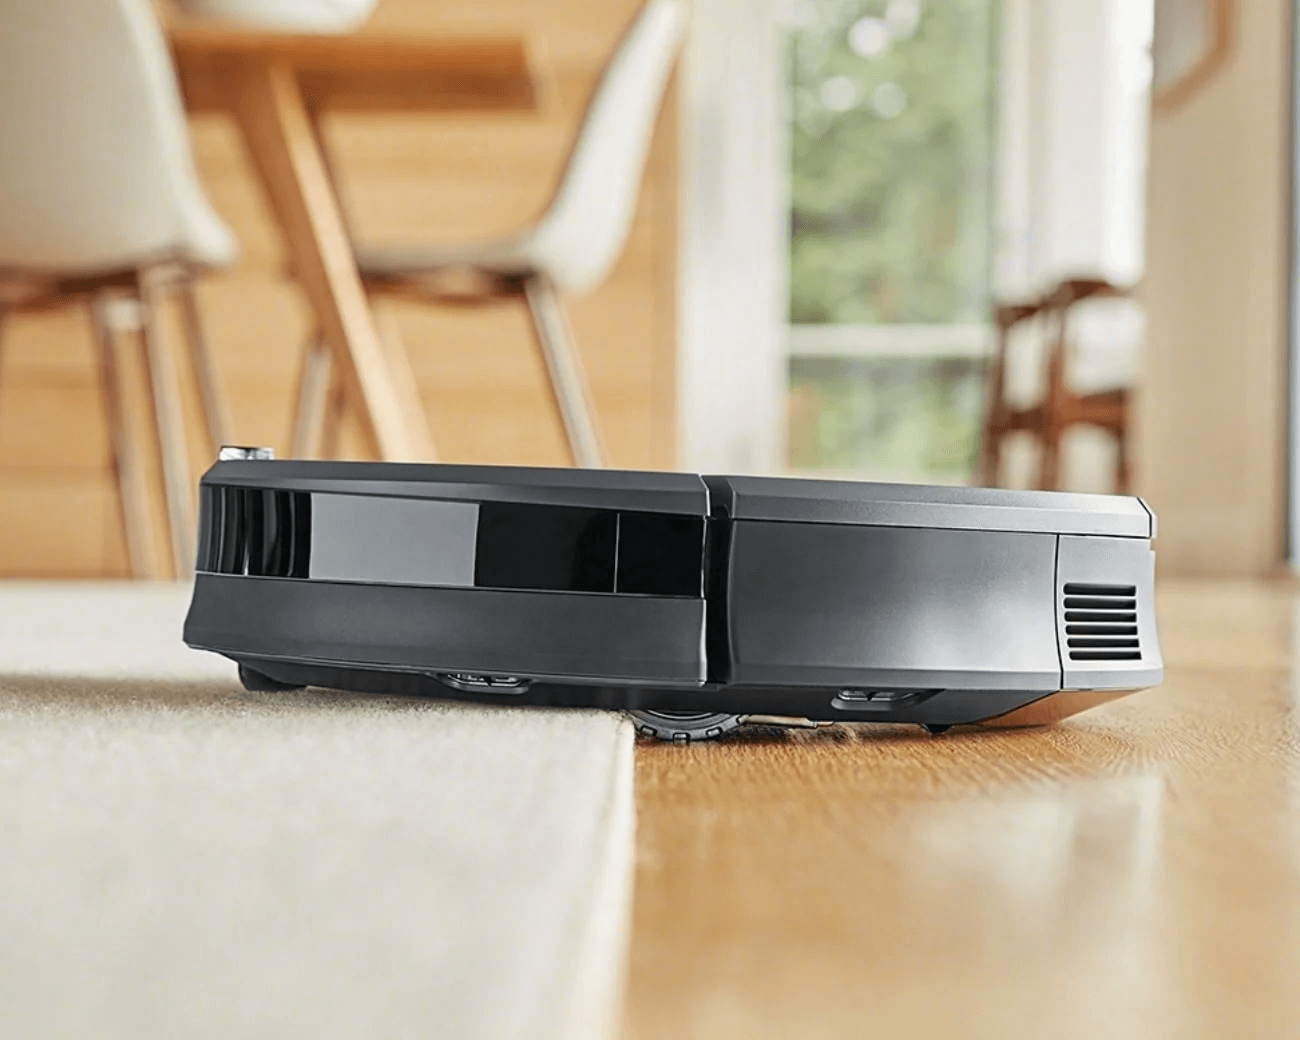
\includegraphics[width=50mm]{image/roomba.png}
  \caption{段差を乗り越える}
  \label{fig:runba}
\end{figure}

したがって、室内移動型のロボットを複数階建ての一軒家などで運用する場合、
複数のフロアで稼働させるためには人間がロボットを移動させるか、別フロアの作業は人間が行う必要がある。
移動させる作業はロボットの重量が増えていくごとに困難になり、
また運用者が高齢になると作業中の事故などが懸念される。
また、人間が代わりの作業を行うとなると、ロボットを導入したメリットを享受できるのが1フロアだけになってしまう。


そこで、車輪で移動を行い、段差の上り下りを車輪に依存せずに行うロボットを開発すれば、
車輪径や車高は別の問題に最適化しつつ、フロア移動が可能になるのではないかと考えた。
\section{研究目的}


\section{研究方法}
\section{スケジュール}
\section{期待される効果}
\section{大学院での抱負}


\end{document}
